\documentclass[tikz,border=6pt]{standalone}
\usepackage[T1]{fontenc}
\usepackage[utf8]{inputenc}
\usepackage{pgfplots}
\usepgfplotslibrary{groupplots}
\usetikzlibrary{calc}
\pgfplotsset{compat=1.18}
\begin{document}
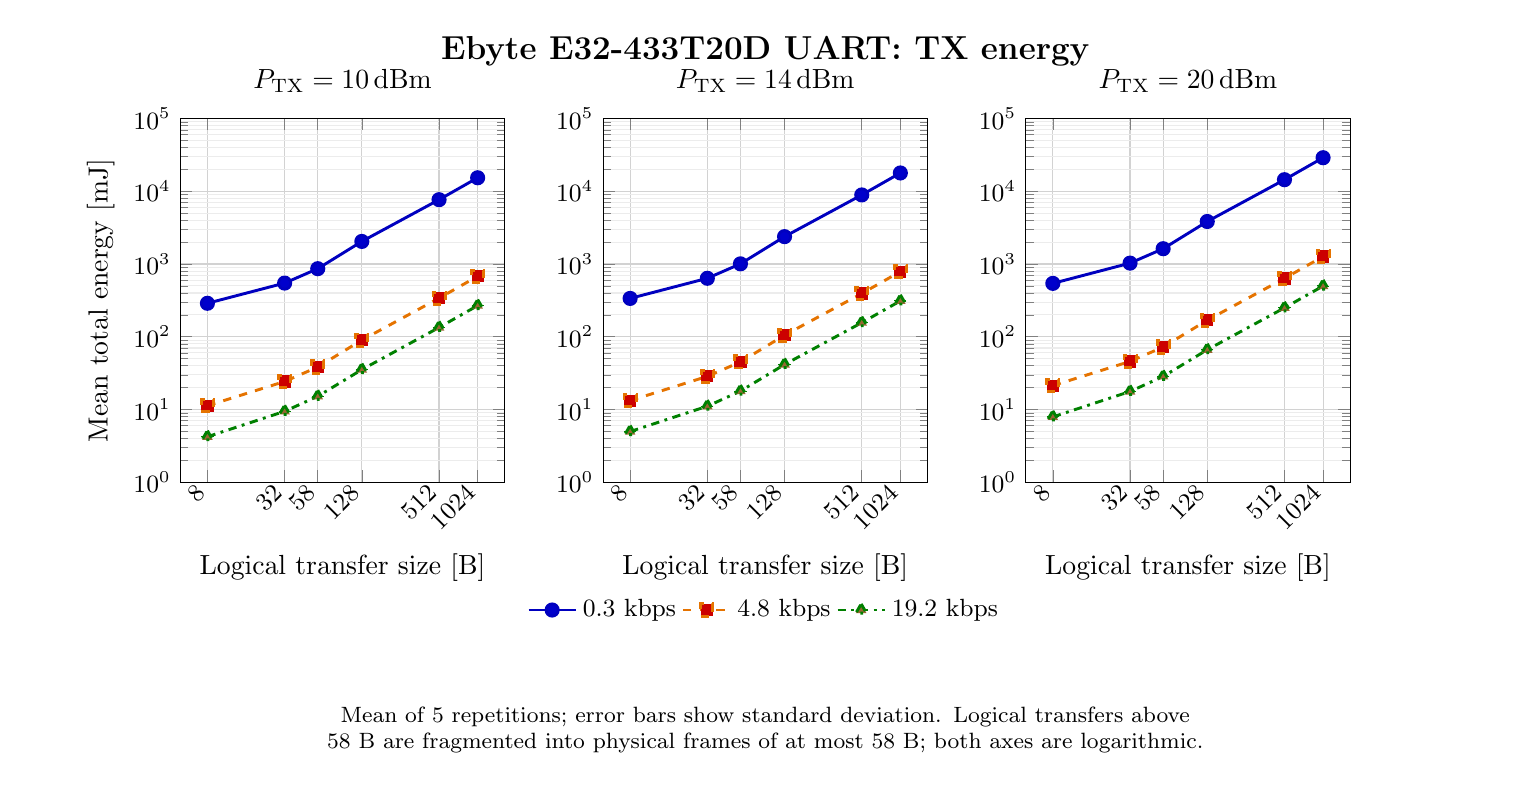
\begin{tikzpicture}
\begin{groupplot}[/pgf/number format/use comma,
  group style={group size=3 by 1, horizontal sep=1.25cm},
  width=5.7cm, height=6.2cm,
  xmode=log, log basis x={2}, ymode=log, log basis y={10},
  ymin=1, ymax=100000,
  xtick={8,32,58,128,512,1024}, xticklabels={8,32,58,128,512,1024},
  x tick label style={rotate=45, anchor=east, font=\small},
  y tick label style={font=\small},
  grid=both, minor grid style={gray!15}, major grid style={gray!35},
  xlabel={Logical transfer size [B]},
  every axis plot/.append style={line width=1.05pt},
  error bars/error bar style={line width=0.35pt},
  legend style={font=\small, draw=none, fill=none, at={(0.5,-0.29)},
    anchor=north, legend columns=-1},
]
\nextgroupplot[title={\(P_{\mathrm{TX}}=10\,\mathrm{dBm}\)}, ylabel={Mean total energy [mJ]}]
\addplot+[
  color=blue!75!black, solid, mark=*, mark size=2.2pt,
  error bars/.cd, y dir=both, y explicit,
] coordinates {
  (8,288.621706) +- (0,0.310786356)
  (32,546.962462) +- (0,0.564098983)
  (58,863.267334) +- (0,0.945942058)
  (128,2045.42671) +- (0,0.560352587)
  (512,7673.09947) +- (0,1.39022557)
  (1024,15357.8682) +- (0,6.44803308)
};
\addplot+[
  color=orange!90!black, dashed, mark=square*, mark size=2.2pt,
  error bars/.cd, y dir=both, y explicit,
] coordinates {
  (8,11.2607652) +- (0,0.00807605154)
  (32,24.2612116) +- (0,0.0186272953)
  (58,38.3574241) +- (0,0.0554699878)
  (128,89.9789604) +- (0,0.0594788881)
  (512,339.219437) +- (0,0.155708243)
  (1024,678.744775) +- (0,0.435433624)
};
\addplot+[
  color=green!50!black, dashdotted, mark=triangle*, mark size=2.2pt,
  error bars/.cd, y dir=both, y explicit,
] coordinates {
  (8,4.22342895) +- (0,0.00577087021)
  (32,9.43036665) +- (0,0.0144202661)
  (58,15.1828328) +- (0,0.0207485812)
  (128,35.3542242) +- (0,0.0327287036)
  (512,134.195872) +- (0,0.0736315671)
  (1024,268.265357) +- (0,0.104506448)
};
\nextgroupplot[title={\(P_{\mathrm{TX}}=14\,\mathrm{dBm}\)}]
\addplot+[
  color=blue!75!black, solid, mark=*, mark size=2.2pt,
  error bars/.cd, y dir=both, y explicit,
] coordinates {
  (8,336.754568) +- (0,0.547273852)
  (32,636.877644) +- (0,1.22206435)
  (58,1006.71938) +- (0,1.27061151)
  (128,2380.72737) +- (0,3.81814455)
  (512,8918.71053) +- (0,11.4376842)
  (1024,17870.6746) +- (0,9.41810834)
};
\addlegendentry{0.3 kbps}
\addplot+[
  color=orange!90!black, dashed, mark=square*, mark size=2.2pt,
  error bars/.cd, y dir=both, y explicit,
] coordinates {
  (8,13.2372393) +- (0,0.0522869754)
  (32,28.5434303) +- (0,0.0433414406)
  (58,45.0703532) +- (0,0.224736565)
  (128,105.195765) +- (0,0.474690327)
  (512,393.180768) +- (0,0.81602771)
  (1024,787.11854) +- (0,0.541205997)
};
\addlegendentry{4.8 kbps}
\addplot+[
  color=green!50!black, dashdotted, mark=triangle*, mark size=2.2pt,
  error bars/.cd, y dir=both, y explicit,
] coordinates {
  (8,4.97394146) +- (0,0.014013205)
  (32,11.0935679) +- (0,0.0530655242)
  (58,17.8862617) +- (0,0.0373392354)
  (128,41.5689917) +- (0,0.197813903)
  (512,156.291786) +- (0,0.597205975)
  (1024,311.15162) +- (0,0.74150084)
};
\addlegendentry{19.2 kbps}
\nextgroupplot[title={\(P_{\mathrm{TX}}=20\,\mathrm{dBm}\)}]
\addplot+[
  color=blue!75!black, solid, mark=*, mark size=2.2pt,
  error bars/.cd, y dir=both, y explicit,
] coordinates {
  (8,542.077683) +- (0,0.476680879)
  (32,1029.33218) +- (0,1.4044938)
  (58,1624.89807) +- (0,2.05573686)
  (128,3846.02637) +- (0,2.94000291)
  (512,14447.2025) +- (0,13.1733198)
  (1024,28958.0312) +- (0,32.4301291)
};
\addplot+[
  color=orange!90!black, dashed, mark=square*, mark size=2.2pt,
  error bars/.cd, y dir=both, y explicit,
] coordinates {
  (8,21.2945275) +- (0,0.0302056589)
  (32,45.8073506) +- (0,0.170395694)
  (58,72.3133997) +- (0,0.237277791)
  (128,169.02978) +- (0,0.553425085)
  (512,634.409172) +- (0,0.949392434)
  (1024,1269.81883) +- (0,0.974012847)
};
\addplot+[
  color=green!50!black, dashdotted, mark=triangle*, mark size=2.2pt,
  error bars/.cd, y dir=both, y explicit,
] coordinates {
  (8,7.91120402) +- (0,0.0101505503)
  (32,17.6863226) +- (0,0.0301411057)
  (58,28.4690745) +- (0,0.0800841039)
  (128,66.3184263) +- (0,0.211907672)
  (512,249.792515) +- (0,0.517092667)
  (1024,498.822931) +- (0,1.06865604)
};
\end{groupplot}
\node[font=\bfseries\large] at ($(group c2r1.north)+(0,0.85cm)$)
  {Ebyte E32-433T20D UART: TX energy};
\node[font=\footnotesize, align=center, text width=18.5cm]
  at ($(group c2r1.south)+(0,-3.15cm)$)
  {Mean of 5 repetitions; error bars show standard deviation. Logical transfers above 58 B are fragmented into physical frames of at most 58 B; both axes are logarithmic.};
\end{tikzpicture}
\end{document}
